\documentclass[12pt,titlepage,french]{article}
\usepackage{babel}
\usepackage{graphicx}
\usepackage[margin=2.5cm]{geometry}
\usepackage{tabularx}
\usepackage[hidelinks]{hyperref}

\usepackage[utf8]{inputenc}
\usepackage[T1]{fontenc}
\pagestyle{plain}

\usepackage{booktabs,makecell,tabu}
\usepackage{float}
\renewcommand\theadfont{\bfseries}

\linespread{1.2}

\begin{document}

\begin{titlepage}
\newcommand{\HRule}{\rule{\linewidth}{0.5mm}}
\center

  
\includegraphics[width=0.45\textwidth]{../ressources/img_logos/logo_polytech.png}\\[1cm]

  
\includegraphics[width=0.45\textwidth]{../ressources/img_logos/logo_taglabs.png}


\HRule \\[0.4cm]
{ \huge \bfseries Description du système \\[0.15cm] }
Classification colorimétrique de nuages de points 3D
\HRule \\[1.5cm]
Ronan Collier,
Mathieu Letrone,
Tri-Thien Truong
\\[1cm]
\today \\ [1cm]
Version 1.0 - Beta
\end{titlepage}

\tableofcontents % table des matières
\newpage
\listoffigures  % table des figures
\newpage
\section{Contexte et problème}

Taglabs est une jeune entreprise créée il y a deux ans par Yan Koch. L’entreprise s’inscrit dans le domaine de la modélisation 3D d’ouvrages. Ils proposent la modélisation et l’exploitation de nuages de points. Toutefois, ils travaillent surtout en interne sur un logiciel « ScanSap ». Le but de ce logiciel est d’exploiter les nuages de points 3D avec efficacité et simplicité inégalées. \newline

L’entreprise travaille principalement avec les acteurs du BTP et de l’industrie sur des opérations de rénovation et de modernisation des ouvrages. Ces opérations nécessitent de s’appuyer sur des plans qui vont servir aux divers corps d’état pour préparer les travaux.\newline

Par le passé, les plans étaient physiques (plans papiers), et sont désormais numériques (plans 2D et maquettes 3D). Ces plans sont malheureusement souvent obsolètes, ce qui est lié aux nombreux petits travaux réalisés au cours de la vie des bâtiments, et qui ne font pas l’objet de mise à jour documentaire. Ceci conduit les entreprises à faire des erreurs dans leurs études techniques, puis des reprises sur site chronophages et coûteuses. \newline

Depuis quelques années, il est possible de faire scanner les bâtiments en 3D et ainsi obtenir un relevé précis sous forme de nuages de points. Le problème rencontré par les entreprises réside dans la difficulté d’exploitation de ces relevés.\newline

\begin{figure}[H]
\center

\includegraphics[width=0.7\textwidth]{./img/exemple_ndp.PNG}
    \caption{\label{} Exemple de nuage de points en 3D}
\end{figure}

Nous pouvons voir ci-dessus, un exemple de nuage de points en 3D, que l'entreprise utilise en tant que données d'entrée. C'est un nuage de points très volumineux, de plus de 22 millions de points. C'est ce type de données que l'entreprise cherche à exploiter au mieux, afin de répondre aux besoins de leurs clients.\newline

TagLabs travaille sur 2 volets :

\begin{itemize}
    \item la conversion du nuage en maquette numérique (CAO / BIM),
    \item l’exploitation du nuage de points tel quel par le biais de fonctionnalités avancées de mesure et de segmentation. \newline
\end{itemize}

C’est ce second volet qui est abordé dans ce projet. \newline

Dans cette optique, l'entreprise souhaite pouvoir intégrer plusieurs fonctionnalités à son système. D'une part, une solution permettant une segmentation basée sur la couleur au sein du ou des nuages de points manipulés. Cette segmentation a pour but de mettre en évidence, isoler les éléments du nuage de point répondant à une plage de couleur demandée. D'autre part, une solution mettant en place une fausse couleur sur un scan (nuage de points) en intensité. Le rôle de la fausse couleur est de mettre en lumière des caractéristiques issu des éléments scannés, et de faciliter la compréhension générale du nuage en y mettant des couleurs. \newline

L'ensemble des fonctionnalités demandées par le client est une demande de recherche algorithmique sur l'implémentation des solutions.

\section{Solution mise en place : vue globale}

Dans cette partie, nous allons présenter l'ensemble des choix que nous avons fait afin de répondre au mieux aux besoins demandés par le client. De plus, nous présenterons la description de la solution conçue pour satisfaire ces besoins.

\subsection{Choix principaux}

Afin de répondre aux besoins, qui sont de pouvoir :
\begin{itemize}
    \item Lire un fichier de données contenant un nuage de point.
    \item Isoler un élément dans le nuage de points, selon sa plage de couleur.
    \item Réaliser de la fausse couleur sur un nuage de points en intensité de gris.
    \item Exporter le nuage de points. \newline
\end{itemize}

Le service proposé doit permettre aux utilisateurs de réaliser ces tâches. Nous avons d'abord défini en tant qu'utilisateurs de la solution, ceux qui utiliseront "ScanSap" qu'il s'agisse de client ou de membre de l'entreprise TagLabs. Ainsi, nous visons des utilisateurs voulant manipuler des nuages de point en 3D. Ces personnes sont équipés de matériels puissants pour faire cela.\newline

N'existant pas d'outil permettant l'ajout direct de fonctionnalités extérieures au sein du logiciel "ScanSap", nous avons décidé avec l'entreprise de réaliser un plugin sur un autre logiciel de manipulation de nuages de points. Le logiciel en question est CloudCompare. Il permet la manipulation et le traitement des nuages. De plus, sa licence open source autorise l'ajout de fonctionnalités tant que nous les livrons aussi en open source. \newline

Cette décision fut prise pour répondre non seulement à l'ensemble des besoins, mais aussi car CloudCompare prend déjà en charge deux besoins, la lecture et l'exportation des scans. En faisant ce choix, nous pouvons nous consacrer à la recherche et la réalisation des autres besoins de la segmentation, et de la fausse couleur.

\subsection{Description de la solution}

Comme dit précédemment, la solution proposée pour répondre à la problématique s'articule autour d'un service de type plugin utilisateur. Le plugin est intégré dans les composants tiers de CloudCompare, il comprend les fonctionnalités de segmentation suivant la plage colorimétrique en RGB, HSV et en valeurs scalaires et du Tone mapping.  \newline

Les utilisateurs pourront y accéder en les sélectionnant dans le menu défilant qui liste les différents plugins présents. Les diagrammes de séquence qui suivent, détaillent et illustrent le fonctionnement de l'expérience utilisateur. \newline

La figure ci-dessous montre la démarche que doit suivre l'utilisateur pour avoir accès au plugin.

\begin{figure}[H]
\center
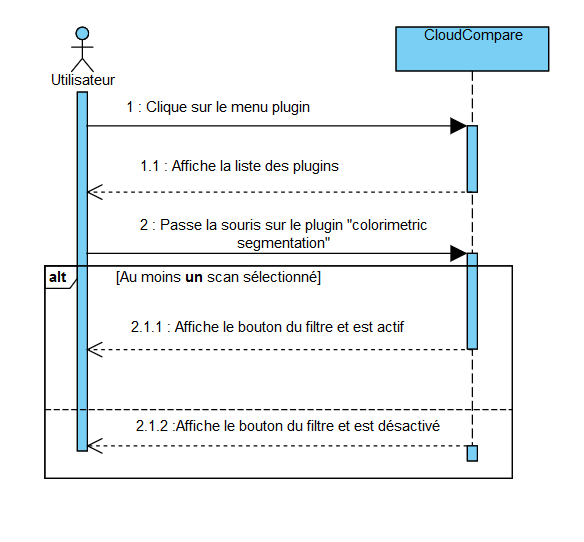
\includegraphics[width=0.65\textwidth]{./img/sequDiagPlugin.PNG}
    \caption{\label{} Diagramme de séquence sur l'accès au plugin}
\end{figure}

La marche à suivre est relativement simple puisque notre plugin s'intègre dans le menu défilant qui répertorie l'ensemble des autres plugins accessibles de CloudCompare. De cette manière, l'utilisateur n'a qu'à le sélectionner et pourra l'utiliser si un ou des nuages ont été choisis pour être traités. \newline

La figure suivante, quant à elle, illustre l'utilisation du plugin, plus particulièrement la segmentation colorimétrique.

\begin{figure}[H]
\center
  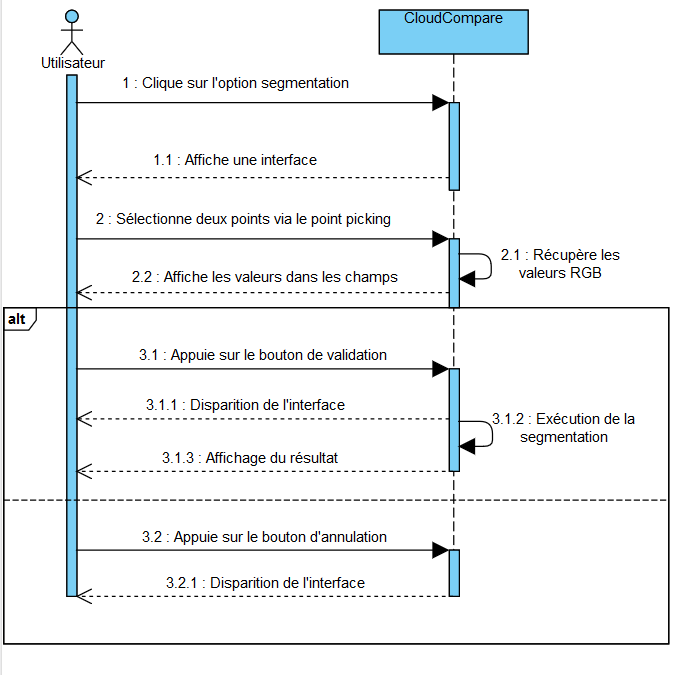
\includegraphics[width=0.65\textwidth]{./img/sequDiagrSegmentation.PNG}
  \caption{\label{} Diagramme de séquence sur l'utilisation de la segmentation}
\end{figure}

L'expérience utilisateur a été revue et s'améliore au fil des retours client à chaque itération. Ainsi, ce diagramme prend en compte les feedbacks de la dernière itération en date, mais sont encore susceptibles d'évoluer jusqu'à la recette. Une fois les étapes de la figure 1 réalisés, une fenêtre apparaît et permet à l'utilisateur de choisir deux points dans le nuage via le point picking de CloudCompare. Ces points serviront pour définir les bornes de la plage colorimétrique des élément qu'il souhaite isoler. Une fois fait, il peut valider son choix via un bouton ou annuler l'opération. \newline

Le tableau ci-dessous présente l'état d'avancement des composants de la solution, en mettant en évidence leur état via un code couleur :
\begin{itemize}
    \item Vert : composant réalisé
    \item Orange : composant en cours de réalisation
    \item Rouge : composant pas encore réalisé
    \item Bleu : composant déjà existant
\end{itemize}

\begin{figure}[H]
\center 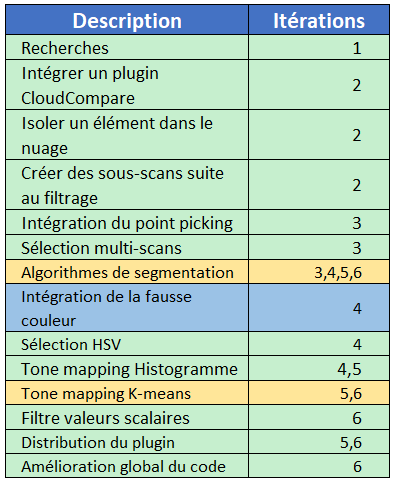
\includegraphics[width=0.4\textwidth]{./img/avancement.png}
  \caption{\label{} Tableau d'avancement global}
\end{figure}

Les composants et tâches planifiés ont évolué au cours de l'avancement du projet.
Certains composants ont été soulevés suite aux feedbacks de nos réunions et discussions avec le client et notre tuteur académique comme le Tone mapping ou le point picking.
D'autres tâches, comme le filtrage HSV et le filtrage avec valeurs scalaires sont apparues pour répondre à la tâche planifiée qu'est l'implémentation de la fausse couleur.\newline

En effet, nous avons remarqué que la fausse couleur était déjà intégrée à CloudCompare.
Ainsi, il n'était plus nécessaire de la développer, mais à la place nous avons vu qu'il était possible de proposer un filtrage directement sur des champs scalaires.
Étant à la fin du projet, on peut noter que l'ensemble des composants listés ont été implémentés et intégrés à la solution. \newline

Il faut aussi noter que nous avons quelques tâches qui n'ont pas été totalement finalisées, notamment le développement d'un algorithme de segmentation, ou encore le Tone mapping avec K-means. Concernant la première tâche, ceci est dû notamment aux difficultés rencontrées pendant l'implémentation, et l'autre est dû au manque de temps.

\section{Description technologique de la solution}

Dans cette partie, nous présenterons les différents composants de l'architecture qui composent notre projet. Nous présenterons également la structure du code, et des différents éléments qui interagissent sur le projet.

Notre solution étant un plugin pour CloudCompare, la principale difficulté technique est la compréhension de la structure de ce logiciel et de son API. \newline

En effet, CloudCompare possède une structuration complexe pour toute personne qui n'est pas habituée à travailler sur des projets C++ d'une telle envergure.

De plus, la documentation possède de nombreuses lacunes, ne présentant pas toutes les classes et n'étant pas à jour.
Il est donc conseillé de regarder le fonctionnement de l'API en naviguant dans les sources du projet.

\subsection{Structure du code source CloudCompare}

Nous présenterons ici la structure du projet CloudCompare, et de l'implémentation de notre plugin.

\begin{figure}[H]
\center
  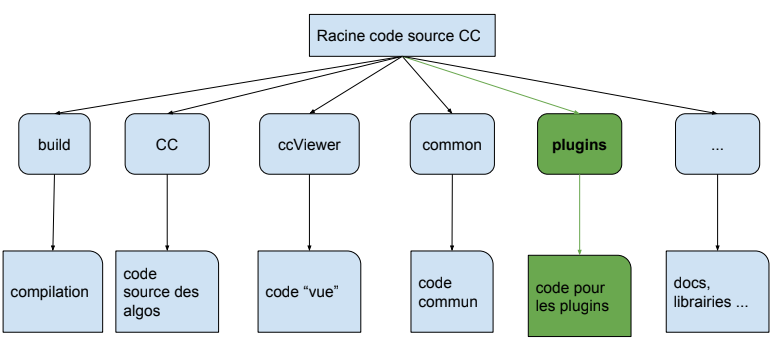
\includegraphics[width=0.8\textwidth]{./img/structure_code.PNG}
  \caption{\label{} Code source du projet CloudCompare}
\end{figure}

Le code source du projet se trouve aux côtés de celui des autres plugins, dans le dossier "plugins" situé à la racine du dossier des sources de CloudCompare (représenté en vert sur la figure ci-dessus). Chaque sous-dossier de ce dossier représente un plugin. \newline

Pour représenter comment les différents composants sont liés ensemble au sein du projet, nous avons utilisé un diagramme de composants. Le plugin se trouve parmi les autres composants tiers à CloudCompare, mais utilise toutes les librairies du cœur de CloudCompare et interface avec le client en passant par le logiciel.

\begin{figure}[H]
\center
  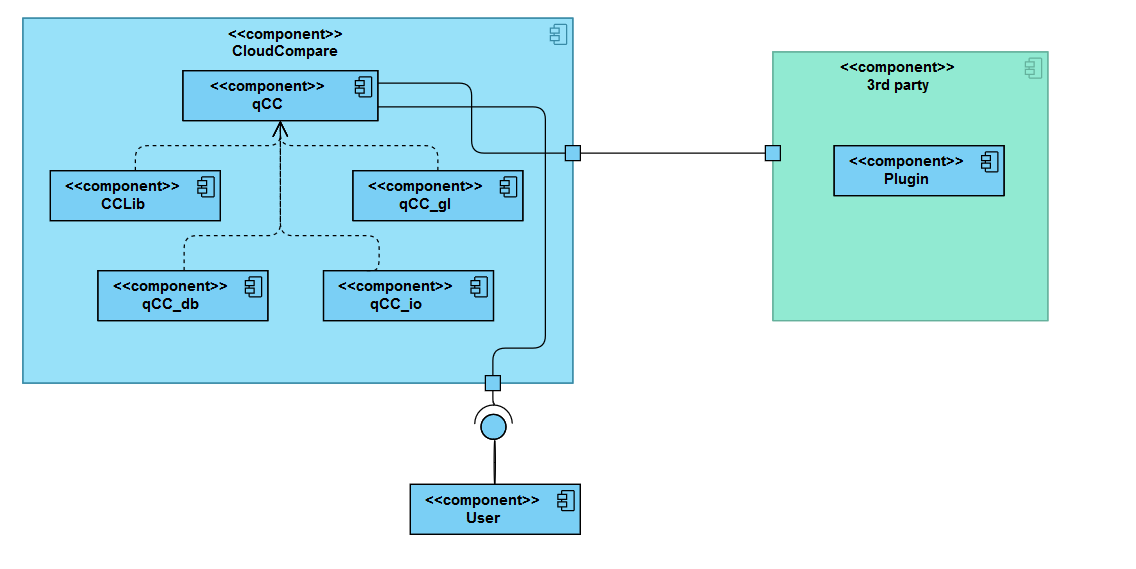
\includegraphics[width=0.9\textwidth]{./img/component_diagr.png}
  \caption{\label{} Diagramme de composants du projet CloudCompare}
\end{figure}

La structure du code source de CloudCompare est organisée pour éviter d'avoir du code éparpillé partout dans le projet original. Nous avons juste à insérer notre code et développer notre propre plugin dans le dossier plugins.

\subsubsection{Projet Cmake}

Le fichier le plus important pour la compilation du projet est le "CMakeLists.txt". En effet, il contient le nom de la classe principale du projet ainsi que tous les fichiers à inclure lors de la compilation.
Si la structure du projet est correcte, et les fichiers correctement configurés, une option sélectionnable apparaît dans CMake.
Il est alors possible de construire le projet pour qu'il soit éditable à l'aide de QtCreator ou tout autre IDE (tel que Visual Studio, en sélectionnant l'option appropriée).

\subsubsection{Intégration du nouveau plugin dans le projet CloudCompare}

Pour chaque plugin, il faut respecter une certaine structure. Dans le projet CloudCompare, il existe une classe template, qui nous a servi pour la création de notre propre plugin. Il est important de bien le construire, afin de pouvoir interagir avec les éléments du logiciel (graphiquement, et sur les données). \newline

Nous avons représenté la structure globale du plugin, avec ce schéma ci-dessous.

\begin{figure}[H]
\center
  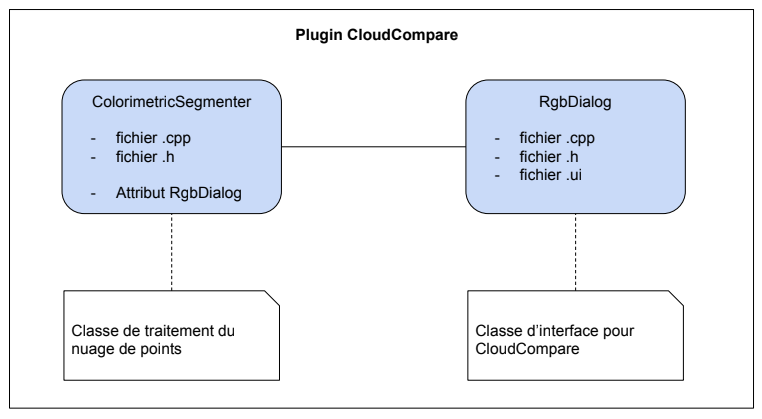
\includegraphics[width=0.7\textwidth]{./img/architecture_plugin.PNG}
  \caption{\label{} Structure de notre plugin}
\end{figure}

Nous pouvons observer que le plugin se compose de deux types de classes. La première, ColorimetricSegmenter, est la classe qui va permettre le traitement des données, et la classe RgbDialog est la classe pour créer l'interface sur CloudCompare d'un type de filtrage. Pour chaque type de filtrage que nous montrerons par la suite, il a fallu créer un nouveau fichier "Dialog".

\subsubsection{Classe de traitement : ColorimetricSegmenter}

Notre classe principale est ainsi nommée "ColorimetricSegmenter". Étant donné que notre projet est en C++, la classe est d'abord représentée sous la forme d'un fichier de type "header", contenant simplement les signatures des méthodes. \newline

Afin de pouvoir interagir avec l'environnement de CloudCompare, il a fallu faire hériter notre classe de la classe "ccStdPluginInterface". Cette dernière est déjà présente dans le projet de base de CloudCompare, et permet de faciliter l'implémentation d'un nouveau plugin. En effet, elle nous permet d'avoir un objet de type "ccMainAppInterface", qui regroupe tous les éléments de la fenêtre, et tous les éléments nécessaires pour interagir sur l'interface. \newline

Cette classe "ColorimetricSegmenter" contient donc tous nos types de filtrage sur le nuage de points. Il contient le code permettant d'effectuer les actions que l'on veut dans le nuage de points au moment où on valide la fenêtre de paramétrage d'un filtrage. \newline

Afin de faire le lien avec l'interface graphique sur CloudCompare (car dans ce fichier, nous avons uniquement la partie "traitement"), il faut aussi penser à initialiser l'attribut de la classe qui correspond à l'objet de l'interface, dans notre cas, c'est l'attribut de type "RgbDialog".

\subsubsection{Classes d'interface}

L'interface graphique de CloudCompare se base sur la bibliothèque Qt. Cette bibliothèque offre plusieurs moyens afin de créer de nouveaux panneaux d'interface, de les intégrer à l'environnement existant, et de les lier à des actions. \newline

QtCreator permet de concevoir graphiquement un panneau au travers d'une interface intuitive en drag\&drop. Le panneau nouvellement créé peut être enregistré au format XML avec l'extension ".ui". Lors de la génération du projet, des fichiers ".h" et ".cpp" sont automatiquement créés par CloudCompare afin de pouvoir ouvrir la fenêtre et manipuler ses champs. \newline

\begin{figure}[H]
\center
  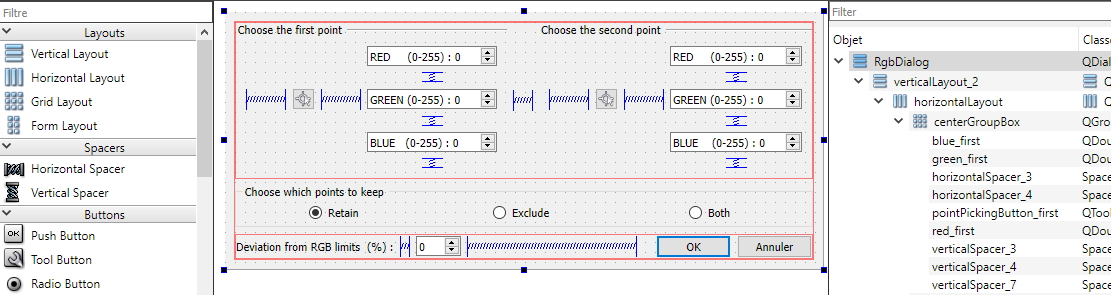
\includegraphics[width=1\textwidth]{./img/qt_creator.PNG}
  \caption{\label{} Exemple QtCreator : RgbDialog}
\end{figure}

Concrètement, nous avons par exemple, un fichier "RgbDialog.ui", créé avec le logiciel Qt Creator. Grâce à ce fichier, en générant le projet, les fichiers "RgbDialog.h" et "RgbDialog.cpp" se créent. Il est ensuite possible d'ajouter des méthodes dans le fichier "RgbDialog.cpp" afin d'ajouter des traitements. \newline

Au niveau de l'interface en elle-même, il s'agit essentiellement de boutons et de champs de texte. Nous avons essayé de faire des interfaces très simples à comprendre et assez épurée.  \newline

Nous avions rencontré des problèmes pour certains types d'écrans (notamment les écrans 4K), où certains composants avaient du mal à s'afficher. C'est pour cela que grâce aux Spacers (représentés en bleu sur l'image ci-dessus), les composants s'adaptent en fonction de la taille de la fenêtre. Chaque utilisateur pourra donc redimensionner la fenêtre selon ses goûts.

\subsubsection{Gestion des actions sur l'interface : Qt}

Les actions utilisateurs sont gérées grâce à Qt au travers de la mécanique des signaux et des slots. Chaque événement, tel que l'ajout d'un nuage de points, est représenté par un slot et un signal. \newline

Notre plugin peut ainsi savoir si l'utilisateur a sélectionné un nuage de points ou non, ou encore s'il clique sur un point. Il est également tout à fait possible de créer des signaux et slots personnalisés. \newline

Chaque action de notre plugin doit être référencée en la déclarant en tant qu'attribut de notre classe, et également dans l'implémentation de la fonction "getActions" de la classe. Un bouton sera alors généré dans l'interface pour chacune de ces actions. La fonction "getActions" permet ici d'établir des conditions préalables sur l'état des boutons, en déterminant par exemple sous quelles conditions ils sont activés ou utilisables. \newline

Dans notre cas, nous avons par exemple ajouté des signaux sur référençant le clic d'un bouton, pour activer un point picking, c'est-à-dire pour activer le mode de sélection de points dans le nuage.

\subsection{Description des algorithmes}

Nous allons présenter ici les différents algorithmes qui nous avons pu développer. Le traitement du nuage de points est composé de deux grandes parties. D'une part, nous avons la segmentation des points dans le nuage. D'autre part, nous devons réaliser nos différents types de filtrage, afin de sélectionner des points qui nous intéressent ainsi que le Tone mapping.

\subsubsection{Algorithme de segmentation}

Notre plugin contient un algorithme de filtrage des points amélioré grâce à une segmentation. Cet algorithme est séparé en deux étapes. Une première consistant à parcourir le nuage de point afin de créer des régions de couleurs similaires, et une seconde étape dite de "raffinement" afin de réunir les régions similaires. \newline

Ainsi, pour chaque point, on regarde ses voisins en ne gardant que ses voisins les plus proches (en terme colorimétrique) afin de former une région. L'algorithme complet est décrit dans une publication de l'université de \cite{B01} Whuan. \newline

La segmentation d'un nuage de points de plusieurs millions de points est un procédé coûteux en temps et en espace. En effet, une approche naïve consisterait à copier les points et les ajouter dans des listes correspondant à des régions. Cependant, la recopie d'une telle quantité de points est trop coûteuse. Il convient donc de travailler par référence en manipulant plutôt les index de ces points.
Afin de réaliser cela, nous utilisons une structure de données fournie par Cloud Compare: le nuage de point par référence (ReferenceCloud). Cette structure se base sur un nuage de point déjà existant et contient un index des points du nuage. On manipule ainsi deux index, un index local (les points du nuage par référence, ajoutés) et un index global (les points du nuage de base). \newline

La recherche des plus proches voisins est également une étape coûteuse en temps. Une autre structure de donnée fournie par CloudCompare fournit les méthodes de recherche du plus proche voisin optimisée pour de multiples appels enchainés. Il s'agit de la structure Octree. Dans cette structure, le nuage est découpé en cellules pouvant se subdiviser en plusieurs autres niveaux de cellules. L'implémentation de cette structure contient la méthode "findNearestNeighborsStartingFromCell", qui réalise la recherche des plus proches voisins dans le nuage à partir d'un point donné. \newline

Bien qu'implémenté, cet algorithme n'a pas été suffisamment testé. Sa complexité étant en $O(n^{2})$, le temps de calcul sur plusieurs millions de points est considérable. Ce problème est dû aux multiples recherches de voisinages de points.

\subsubsection{Conversion RGB à l'espace colorimétrique CIELAB}

Compte tenu de l'impact du mouchetage sur le nuage de point, il s'agissait du problème le plus important à palier afin d'obtenir une segmentation colorimétrique la plus rigoureuse.
C'est pourquoi, nous nous sommes tournés vers un autre espace colorimétrique que le classique RGB.
Le CIELAB ou lab, est un espace où la luminance et la chrominance sont dissociés, or le problème réside dans des variations de la luminance, mais dans une même gamme de couleurs.
Dans le cas du lab, il suffirait de ne prendre en compte seulement la chrominance.
\newline

\begin{figure}[H]
\center
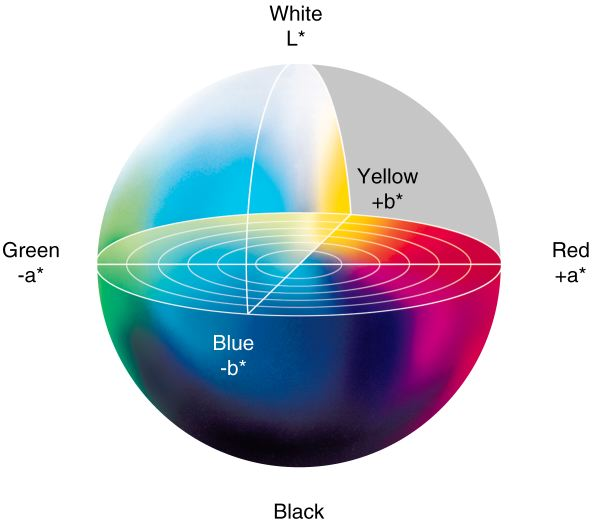
\includegraphics[width=0.4\textwidth]{./img/CIELAB.png}
    \caption{\label{} Répresentation de l'espace CIELAB}
\end{figure}

Cependant, l'utilisation du lab a des désavantages, il faudra réaliser la conversion de RGB à XYZ puis de XYZ à lab avant de pouvoir réaliser le processus de segmentation et ceci sur l'ensemble des points qui composent le nuage.
De plus, la représentation lab requière plus d'espace mémoire. En effet, lors d'un jeu de tests, on a pu constater qu'entre segmentation naïve RGB et CIELAB, le ratio de temps d'exécution était environ de 15.
Après discussion avec le client, il a été convenu de nous concentrer sur d'autres algorithmes et de chercher vers d'autres espaces colorimétriques où la conversion est moins complexe.

\subsubsection{Filtrage via les valeurs RGB}

Notre première solution développée pour obtenir un filtrage, est d'utiliser l'espace colorimétrique le plus commun : le RGB. Dans un nuage de points en couleur, chacun de ces points possède des valeurs de rouge, vert et bleu, de 0 à 255 en intensité.

\begin{figure}[H]
\center
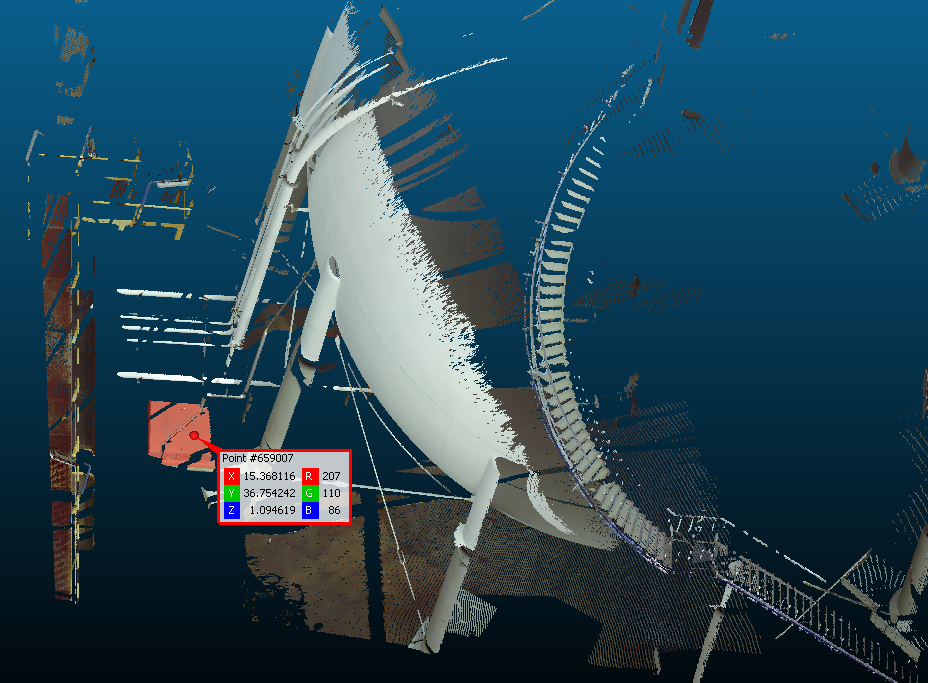
\includegraphics[width=0.5\textwidth]{./img/exemple_rgb.PNG}
    \caption{\label{} Exemple des valeurs RGB d'un point rougeâtre}
\end{figure}

Nous pouvons voir dans cet exemple, les valeurs RGB d'un point qui a été sélectionné via le point picker intégré au logiciel CloudCompare. Les valeurs en intensité sont respectivement 201-112-93. \newline

Notre première idée a donc été d'exploiter ces trois valeurs, et d'avoir un premier filtrage du nuage. Pour ce faire, nous avons réalisé un algorithme consistant à sélectionner uniquement les points qui ont des valeurs RGB proches d'un point dans le nuage. Dans nos premières itérations, nous nous basions uniquement sur la sélection d'un point, pour en définir des bornes RGB qui vont constituer notre plage de points à garder, grâce à un pourcentage d'écart. Suite à des réunions avec le client, une autre solution alternative a été de sélectionner deux points, pour directement définir nos bornes. \newline

Pour cela, nous avons développé dans un premier temps, l'interface utilisateur. Cette dernière est composée de deux points à renseigner, par leurs valeurs RGB. Afin de simplifier l'utilisation du plugin, nous avons intégré un bouton afin de sélectionner un point directement sur le nuage, et qui va ensuite renseigner les valeurs RGB du point sélectionné automatiquement. Il est aussi possible de choisir les points que l'utilisateur veut garder. Le choix de l'option "Retain" permet à l'utilisateur de créer un sous-scan où les points affichés seront les points qui sont à l'intérieurs des bornes. Inversement, l'option "Exclude" va permettre de créer un sous-scan avec les points qui seront hors de l'intervalle choisi. Enfin, la dernière option "Both" va permettre de réaliser les deux options. Nous aurons donc à la fin, deux sous-scans où la somme va permettre de retrouver le scan original. Nous avons enfin un champ afin d'écarter les limites de nos bornes RGB, pour accepter des points qui sont proches des bornes renseignées.

\begin{figure}[H]
\center 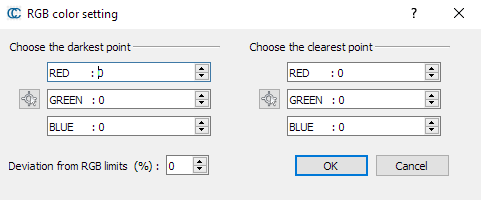
\includegraphics[width=0.7\textwidth]{./img/ui_filter_rgb.png}
  \caption{\label{} Interface filtrage RGB}
\end{figure}

Après le renseignement des différents paramètres, et la validation de la fenêtre via le bouton "OK", le plugin va recalculer les bornes si un pourcentage d'écart à été renseigné. Une fois ces nouvelles bornes calculées, il reste donc à parcourir l'ensemble des points du nuage, et de vérifier pour chaque point, si ses valeurs RGB sont à l'intérieur des bornes. Les points qui respectent cette condition sont gardés dans une liste de points, et les autres seront stockés dans une autre liste. Ces deux listes vont nous permettre de créer des sous-scans sur CloudCompare, selon le choix sélectionné par l'utilisateur.

\begin{figure}[H]
\center

\includegraphics[width=1\textwidth]{./img/rgb_avant_apres.PNG}
\caption{\label{} Filtrage RGB rouge : avant / après}
\end{figure}

Malgré une solution qui semble fonctionner, nous pouvons quand même ressentir les limites de cette méthode. En effet, en utilisant uniquement l'espace colorimétrique RGB, nous sommes limités pour établir des vraies bornes qui permettent de séparer les couleurs plus nuancées. En effet, la qualité du filtrage dépend en grande partie des points que l'utilisateur aura sélectionné, et reste très vague en utilisant uniquement des bornes sur les valeurs RGB. C'est donc pour cela que nous avons utilisé un autre espace colorimétrique, le HSV, qui nous fournira des informations sur la teinte, la saturation et la valeur d'un point.

\subsubsection{Filtrage via l'espace colorimétrique Hue-Saturation-Value (HSV)}

Afin d'avoir plus de précisions sur la sélection de plages de couleurs, nous avons donc décidé d'utiliser l'espace colorimétrique HSV (Teinte, Saturation, Valeur en français). Cet espace nous semble plus intéressant que du simple RGB, notamment car dans le cas du RGB, la teinte d'une couleur va être définie par l'ensemble des trois composantes. Pour le HSV, c'est uniquement la composante "Teinte" qui va la définir. Grâce à cela, nous allons pouvoir définir des bornes en utilisant uniquement une variable, au lieu de trois. De plus, il va être plus facile de détecter un point avec une couleur plus ou moins sombre grâce aux deux autres composantes.

\begin{figure}[H]
\center
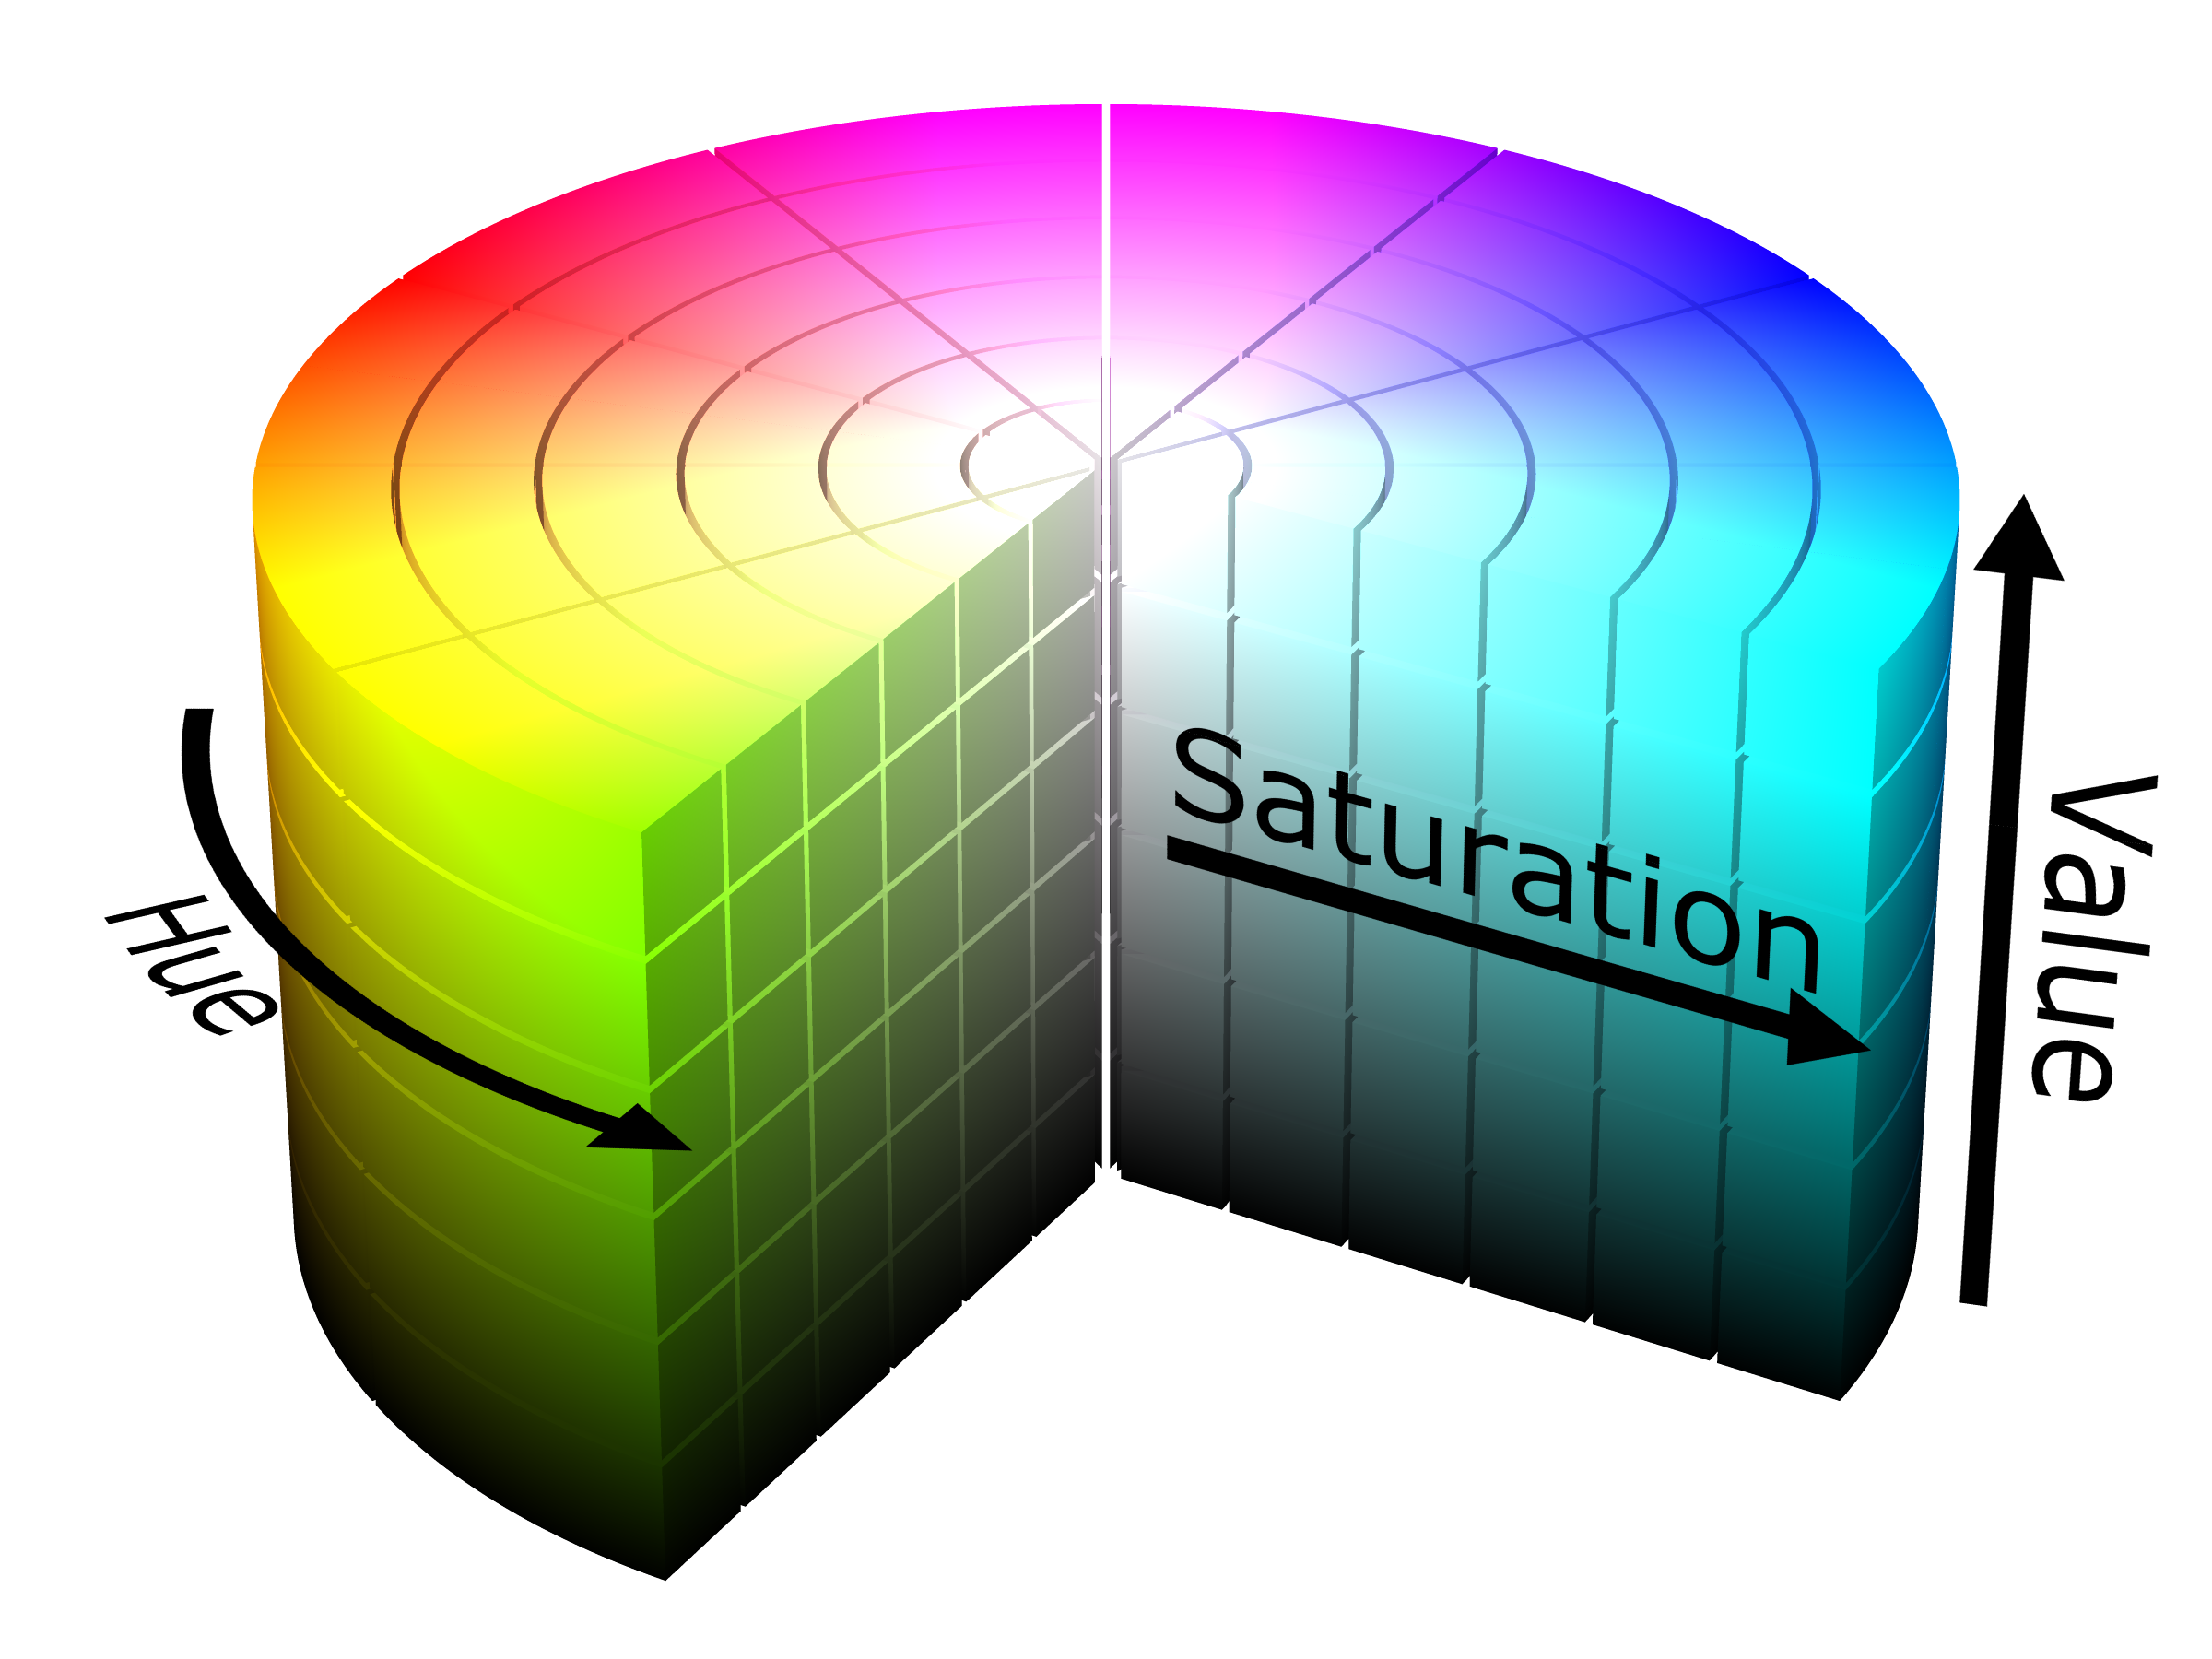
\includegraphics[width=0.3\textwidth]{./img/HSV.png}
\caption{\label{} Description de l'espace colorimétrique HSV}
\end{figure}

La teinte va nous permettre de définir la couleur du point, entre 0 et 360 degrés. La saturation et la valeur, en pourcentage, nous donnent respectivement des informations sur la pureté de la couleur (0 est égal à pas de couleur, donc en nuances de gris entre le blanc et le noir, et 100 pour une couleur vive), et l'intensité lumineuse (0 pour du noir, 100 pour une couleur très claire). \newline

Pour utiliser cet espace colorimétrique, il faut convertir nos valeurs RGB d'un point, en HSV. En effet, les points dans le nuage sur CloudCompare, ont des valeurs uniquement avec du RGB. Il n'y avait pas de conversion RGB en HSV disponible sur le code source du projet CloudCompare, nous avons donc dû le faire nous-même. La conversion est nommée rgb2hsv dans le fichier HSVDialog.cpp. \newline

La description de l'algorithme de conversion est disponible ici \cite{B02}. \newline

Une fois la conversion faite, nous allons pouvoir utiliser nos trois nouvelles composantes pour établir nos bornes de couleurs. Nous avons réalisé nos bornes en plusieurs étapes : \newline

Tout d'abord, nous avons commencé par analyser la composante de la saturation. Cette dernière nous permet nous dit si la couleur est vive (très "coloré"), ou pâle. Nous avons considéré qu'une saturation entre 0 et 25, sur 100, donnait une couleur pâle, donc une couleur dans les nuances de gris. Grâce à cela, nous n'avons donc pas besoin d'analyser la teinte, puisque nous savons que la couleur sera grise. \newline

Dans le cas d'une couleur grise, nous pouvons donc analyser la composante de la valeur. Ici, nous avons remarqué qu'il est donc possible de distinguer 3 couleurs principales : noir, gris et blanc. Nous avons donc défini le noir comme étant une valeur entre 0 et 25, gris pour une valeur entre 26 et 60, et blanc pour une valeur entre 61 et 100. \newline

Dans le cas où nous avons une couleur non-grise, nous avons décomposé l'analyse de la valeur en deux parties seulement : une couleur noire et les autres couleurs. \newline

Une couleur noire aura une valeur entre 0 et 25. Il n'y aura donc pas besoin d'analyser la teinte. Dans le cas contraire, il faudra l'analyser pour séparer les gammes de couleurs. \newline

Concernant la dernière composante, qui est la teinte, nous nous sommes aidé du cercle chromatique, ci-dessous.

\begin{figure}[H]
\center
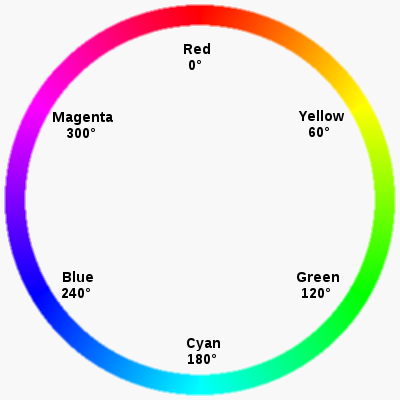
\includegraphics[width=0.3\textwidth]{./img/cercle_chromatique.png}
\caption{\label{} Cercle chromatique}
\end{figure}

Les plages de couleurs que nous avons fixées sont donc les suivantes :

\begin{itemize}
    \item Rouge : $0 \leq teinte \leq 30$
    \item Jaune : $30 < teinte \leq 90$
    \item Vert : $90 < teinte \leq 150$
    \item Cyan : $150 < teinte \leq 210$
    \item Bleu : $210 < teinte \leq 270$
    \item Magenta : $270 < teinte \leq 330$
    \item Rouge : $330 < teinte \leq 360$ \newline
\end{itemize}

Nous pouvons donc maintenant classifier nos points selon nos composantes HSV. Il ne nous reste donc qu'à ajouter les points qui sont de la même catégorie que le point sélectionné. \newline

Au niveau de l'interface, elle est très similaire à celle du RGB, en ajoutant les trois nouvelles composantes du HSV.

\begin{figure}[H]
\center 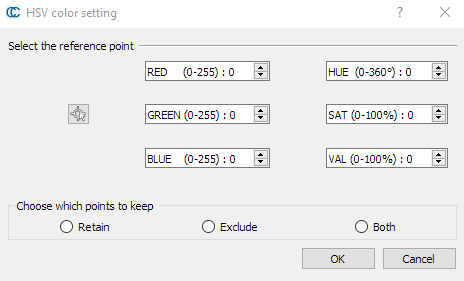
\includegraphics[width=0.6\textwidth]{./img/ui_filter_hsv.PNG}
  \caption{\label{ui_hsv} Interface filtrage HSV}
\end{figure}

Il est possible d'utiliser le point picking afin de choisir directement un point sur le nuage, ce qui va remplir les trois champs RED / GREEN / BLUE. Lorsque un de ces trois champs est modifié, les trois autres champs HUE / SAT / VAL sont automatiquement modifiés. Il est aussi possible de modifier les valeurs directement en modifiant un des champs.

Ci-dessous, un exemple de ce filtrage, identique à celui pour le RGB :

\begin{figure}[H]
\center
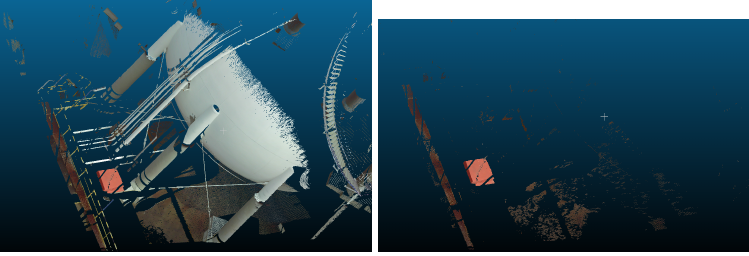
\includegraphics[width=1\textwidth]{./img/hsv_avant_apres.PNG}
\caption{\label{application_hsv} Filtrage HSV rouge : avant / après}
\end{figure}

Nous remarquons une amélioration au niveau de la sélection de tous les points rougeâtres, mais on remarque aussi qu'il y a plus de résidus. En effet, il est difficile de distinguer des points sombres de l'objet rouge que l'on veut sélectionner, des points résidus rougeâtres à cause de l'ombre. \newline

Un autre exemple sur un autre nuage de points va nous permettre de mieux voir les différences. Ci-dessous, nous allons récupérer les points blancs (RGB:255/255/255) :

\begin{figure}[H]
\center
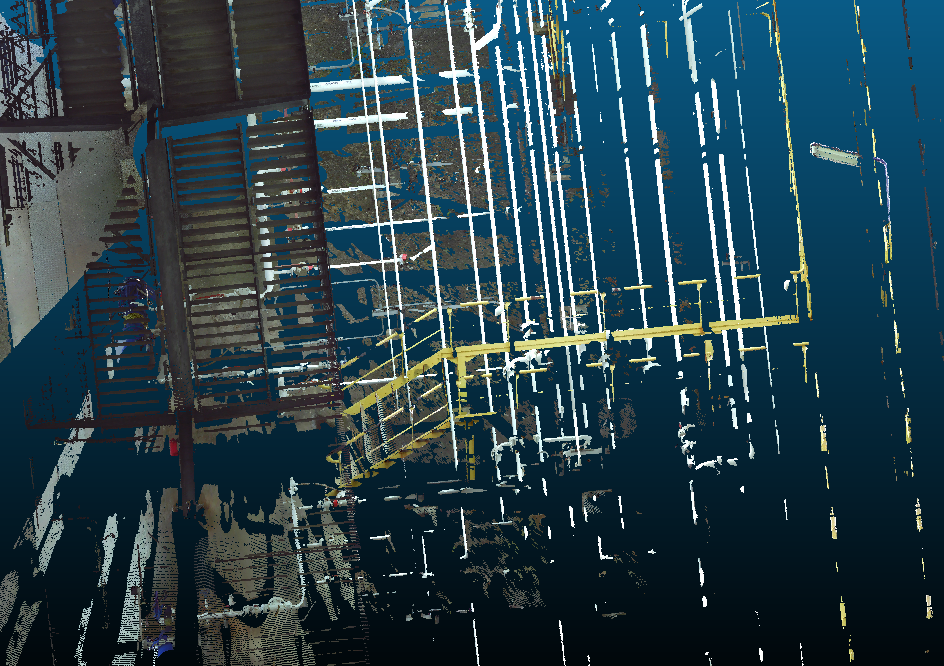
\includegraphics[width=0.5\textwidth]{./img/1_white.PNG}
\caption{\label{} Filtrage blanc : avant}
\end{figure}

\begin{figure}[H]
\center

\includegraphics[width=1\textwidth]{./img/hsv2_avant_apres.PNG}
\caption{\label{} Filtrage RGB blanc et HSV blanc}
\end{figure}

Nous remarquons donc une nette amélioration au niveau de la sélection des tuyaux blancs, surtout pour les tuyaux qui ont une couleur blanche mais avec un peu d'ombre. Même si on obtient des résidus, nous pouvons maintenant récupérer avec plus de précision les points que nous voulons. Les limites de cette méthode sont que les plages de couleurs sont fixes dans le code. Il serait possible d'afficher un mode "avancé" pour l'utilisateur, afin qu'il puisse définir lui-même ses bornes. Après discussion avec les demandes du client, cette option étant facultative et avec un manque de temps sur le projet, nous n'avons pas développé cette partie.

\subsubsection{Filtrage via la valeur scalaire}

Il s'agit d'une fonctionnalité ajoutée à posteriori compte tenu de l'avancement du projet. En effet, il était initialement prévu d'ajouter une fonction permettant de générer de la fausse couleur pour un nuage de points en nuances de gris. Au cours du développement, nous nous sommes aperçu que cette fonctionnalité était déjà présente. Il était par conséquent devenu inutile d'en redévelopper une. Il manquait cependant un outil de filtrage pour ce type de nuage de points. Nous avons donc ajouté un système de filtrage par valeur scalaire. La valeur scalaire correspond à une valeur d'intensité représentée sous format décimal avec une valeur allant de 0 à 1. \newline

Nous nous sommes basés sur la même interface que pour le filtrage RGB. L'utilisateur est invité à renseigner la valeur du point le plus "clair"(une valeur plus proche de 1) et la valeur du plus "foncé" (une valeur plus proche de 0). Il est toujours possible de déterminer ces valeurs en effectuant un point-picking. Un pourcentage d'écart peut être renseigné et recalculera en conséquence les bornes. On peut également choisir si on désire sélectionner les points compris dans l'intervalle de valeurs, ou au contraire ceux qui n'y sont pas inclus. Une fois ce paramétrage réalisé, le nuage est segmenté et un nouveau sous-nuage est créé. Ci-dessous, un exemple de ce filtrage sur les points avec une forte intensité:

\begin{figure}[H]
\center 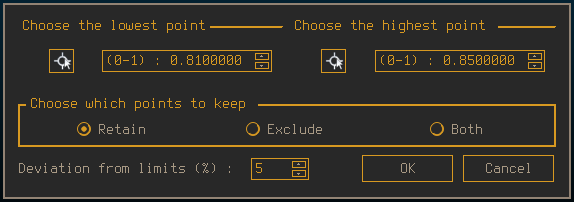
\includegraphics[width=0.6\textwidth]{./img/scalar_menu.png}
  \caption{\label{} Interface filtrage scalaire}
\end{figure}

\begin{figure}[H]
\center
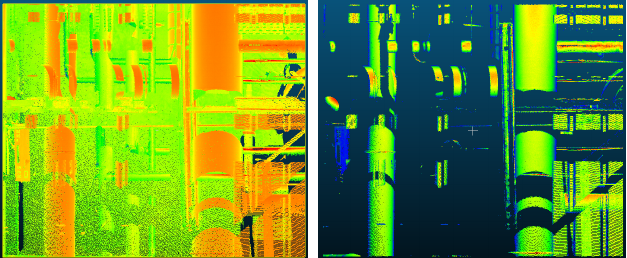
\includegraphics[width=0.9\textwidth]{./img/scalaire_avant_apres.png}
\caption{\label{} Filtrage scalaire : avant}
\end{figure}

Afin de pouvoir distinguer les intensités plus facilement sur l'exemple, nous avons choisi d'appliquer une fausse couleur. Les points de fortes intensités tendent vers le rouge, les plus faible, vers le vert. On peut voir sur le résultat que les points se rapprochant le plus du rouge avant le filtrage sont sélectionnés. Ce qui correspond aux attentes. On pourra noter qu'une nouvelle échelle de couleur est réalisée par CloudCompare, les points n'ont donc plus la même correspondance de couleur.

\subsection{Tone mapping}

Dans l'optique d'avoir une meilleure visualisation des éléments du nuage de points, nous avons ajouté un processus permettant de restreindre la palette de couleurs au sein d'un scan. Ceci a donc pour but de limiter les variations d'intensité imputées par les fusions de scans, qui compose le nuage. Ce processus est analogue à la quantification d'image, deux algorithmes, on était implémentés dans notre solution :

\begin{itemize}
    \item Algorithme par segmentation de l'histogramme
    \item Algorithme K-means
\end{itemize}

L'algorithme de segmentation de l'histogramme scinde chaque composante de l'espace RGB, suivant un coefficient donnée par l'utilisateur.
Pour un N donné, on obtiendra une grille de $Q\times Q \times Q$ cubes / partitions qui engendreront une palette de $Q^3$ couleurs.
\newline

Pour chaque partition, on cherche et attribue chaque point du nuage à celle qui lui est propre. Une fois fait,
on calcule la couleur moyenne de toutes les partitions et on affecte les couleurs obtenues aux points correspondants.
\newline

 \begin{figure}[H]
\center
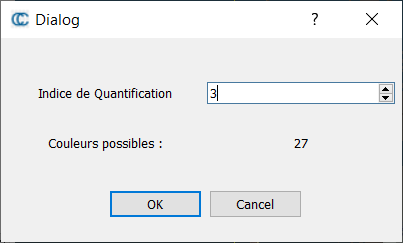
\includegraphics[width=0.5\textwidth]{./img/HistogramDialog.png}
\caption{\label{} Interface quantification par histogramme}
\end{figure}

L'image ci-dessus montre l'interface utilisateur pour la quantification par l'histogramme.
Une spinBox permet à l'utilisateur de choisir le coefficient dans une amplitude de 1 à 255.
 Le champ sur le nombre de couleurs de la palette après exécution se met à jour à chaque valeur changée dans l'indice. Cela permet à l'utilisateur de se projeter et de choisir l'indice qui lui convient le mieux. Une fois le paramétrage réalisé, un nouveau sous-nuage est créé. L'image ci-dessous illustre les résultats obtenus en faisant varier le coefficient.

\begin{figure}[H]
\center
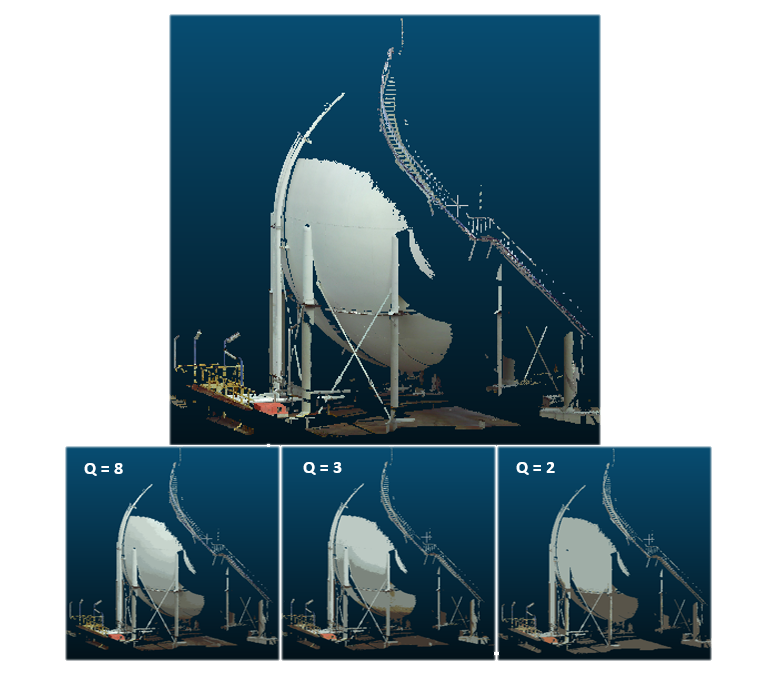
\includegraphics[width=0.75\textwidth]{./img/ExpToonMapping.png}
\caption{\label{} Exemples du Tone Mapping}
\end{figure}

Les limites de cette méthode résident dans les couleurs moyennes.
l'espace RGB n'est pas l'espace colorimétrique le plus adéquat pour générer une couleur moyenne pertinente, mais permet d'éviter le temps d'exécution d'une double conversion.
La seconde limite est le fait que cette méthode peut générer des couleurs qui n'étaient pas présentes à l'origine dans le nuage.
\newline

L'algorithme K-means est connu dans la quantification d'images.
Comme pour l'algorithme de segmentation, il aurait été intéressant de travailler par référence afin de limiter l'utilisation en mémoire.
Cependant, la structure "ReferenceCloud" de CloudCompare, n'a pas accès aux couleurs des points, c'est pourquoi elle n'a pas été utilisée.
Bien que l'algorithme K-means doit se terminer lorsqu'il n'y a plus de variation entre deux itérations, une limite d'itérations a été mise afin que l'utilisateur puisse obtenir un résultat dans un temps modéré.
\newline

Hélas, certains risques résident dans l'algorithme K-means, le risque de rester coincé dans un minimum local. L'autre biais est que le résultat obtenu dépend grandement des points pris à l'initialisation.

\section{Conclusion et perspectives}

Pour conclure sur ces itérations, de façon générale, nous avons pu suivre en grande partie ce que nous avions prévu sur le cahier des charges. La majorité des Users Stories ont été développés et validés par le client. Arrivant à la fin du projet, nous avons pu améliorer ce que nous avions développé dans la version alpha, et terminer les tâches en cours.\newline

Durant la première itération, nous avons de nombreuses questions sur le développement de notre projet. Nous avions notamment le choix du langage, la façon de développer nos algorithmes, l'implémentation, etc. C'était une itération où nous n'avions pas produit de contenu direct pour le client, mais nous avions pu partager nos recherches et de nos choix. Nous avions donc décidé de développer notre solution en C++, avec un plugin CloudCompare. \newline

La recherche d'algorithmes de segmentation nous a permis de gagner du temps sur l'implémentation, afin d'éviter de changer entre phases de recherche, et phases d'implémentation, sur une même itération. Ainsi, cela nous permettait de mieux se concentrer sur la phase d'implémentation. \newline

Toutefois, nous avons quand même pris du retard notamment sur la deuxième et troisième itération. Lors de la deuxième itération, nous pensions que nous pourrions avoir une meilleure base de notre plugin sur CloudCompare, afin de pousser l'implémentation des algorithmes de segmentation. Malheureusement, nous avions rencontré des difficultés par rapport à la création d'un nouveau plugin. Ce temps perdu a donc impacté le développement de la troisième itération, qui consistait à l'amélioration de ce que nous avions développé, et l'implémentation de nouveaux algorithmes. \newline

Lors de la troisième itération, nous avions préféré nous concentrer sur l'amélioration de notre code par rapport à l'implémentation de nouvelles fonctionnalités. Il nous semblait important d'avoir une structure stable et facile à maintenir pour la suite du projet. Grâce à cela, nous avons maintenant un plugin indépendant aux autres, qui est totalement fonctionnel, et auquel on peut aisément ajouter de nouveaux algorithmes de segmentation. \newline

De plus, nous nous sommes efforcés de prendre en compte le feedback du client, afin d'améliorer notre solution par rapport à son utilisation. Ici, ils s'agissait principalement de retours en rapport à l'interface des algorithmes de segmentation. Nous avons apporté des modifications notamment sur le point picking, très important pour faciliter l'utilisation de notre plugin (au lieu de rentrer manuellement les valeurs à filtrer), ou encore des changements sur la plage de couleur à prendre, etc. \newline

Nous avions rencontré beaucoup de difficultés pour fournir la première version du projet à notre client. Il s'agissait notamment de problèmes de compatibilité des versions, par rapport au logiciel CloudCompare, Qt, ou encore la version du SDK de windows. En effet, nous compilions avec une version plus récente de Visual Studio (2019), qui utilisait donc une version SDK Visual Studio plus récente que les machines de notre client. Le seul moyen de savoir d'où venait le problème était de tester différentes solutions de notre côté, puis de les fournir au client afin qu'il puisse réaliser les tests. En prenant en compte les délais de communication, nous avions perdu du temps. \newline

Une fois ce problème résolu, il a nous été assez facile d'avancer sur le projet, tout en prenant en compte le feedback du client qui pouvait utiliser le plugin pour des cas réels. \newline

Même si l'ensemble des tâches a été validé, le projet peut encore être améliorable. En effet, nous pouvons par exemple envisager une version "avancée" du filtrage HSV, pour qu'un utilisateur plus expérimenté puisse affiner sa sélection de points. \newline

Ce projet a à terme vocation à être un plugin qui fera partie de la bibliothèque de plugins de CloudCompare. Un contact a déjà eu lieu avec M. Daniel Girardeau-Montaut, afin de discuter dans un premier temps sur les règles à respecter. \newline

Globalement, c'est un projet transversal qui s'est bien déroulé, et a été très enrichissant de par les connaissances acquises dans le domaine des nuages de points. Nous avons pu découvrir une jeune entreprise qui cherche à innover dans ce domaine, et nous avons eu l'occasion de communiquer avec le créateur du logiciel CloudCompare, qui est considéré comme un logiciel majeur pour le traitement de nuage de points 3D.

\newpage
\section{Annexes}

Les annexes contiendront tout ce qui ne concerne pas directement la description du système. Nous allons décrire le déroulement du projet transversal, et réalisant une rétrospection sur nos itérations. De plus, nous fournirons le rapport de recette.

\subsection{Déroulement du projet}

Il est important de faire un retour sur le déroulement du projet, afin de savoir ce que nous avons bien réalisé, les difficultés que nous avons rencontrés, nos méthodes de travail, etc. En effet, cela nous permettra d'améliorer nos démarches pour mener à bien ce projet.

\subsubsection{Vision globale du projet}

D'un point de vu global sur le projet, nous avons rencontré certaines difficultés, mais aussi appris beaucoup par rapport au fonctionnement d'un projet agile. \newline

Tout d'abord, il a été difficile d'estimer notre charge de travail. Comme il s'agissait de notre premier vrai projet en lien avec une autre entreprise, et d'une aussi grande envergure (durée d'un an), il nous fallait en quelque sorte jauger notre capacité de travail et évaluer les tâches à réaliser. \newline

Certaines tâches furent plus difficiles à réaliser, par rapport à nos prévisions. Par exemple, nous pouvons citer l'implémentation d'un nouvel algorithme de segmentation, plus complexe, ou encore l'implémentation d'un point picking. Le temps prévu à consacrer sur ces types de tâches n'était pas assez important, car nous avions mal pris en compte les autres tâches en parallèle, hors projet. Ces autres tâches étaient notamment d'autres projets sur de courtes durées, devoir surveillées, oraux, etc. \newline

Nous nous sommes aussi rendu compte que les itérations se déroulent très vite. Pour chaque itération, nous étions surpris par le fait qu'un mois s'était passé. Grâce aux réunions planifiées avec le client et le tuteur académique, nous pouvions toutefois garder une bonne dynamique pour respecter les deadlines. \newline

De plus, la mise en situation d'un projet agile nous a fait prendre conscience de l'importance de garder le client au courant, afin d'avancer correctement par rapport aux besoins de celui-ci. Mais pour cela, il faut rédiger de nombreux rapports. Ce sont des tâches qu'il ne faut pas sous-estimer, puisque cela demande beaucoup de temps. Même si les réunions aident à transmettre l'avancement du projet et des tâches réalisées, il faut aussi écrire formellement dans un rapport l'avancement pour garder une trace de ce qui a été fait. \newline

La dynamique de rédaction des rapports d'itération, et des rapports hebdomadaires, est difficile à maintenir. En effet, nous avions eu parfois des difficultés à suivre le rythme des rapports hebdomadaires. Malgré tout, cela reste nécessaire notamment pour avoir un historique de l'avancement des tâches, et des heures passées sur chacune d'entre elles.

\subsubsection{Comparaison de la planification des itérations}

Nous avons aussi réalisé un comparatif de la planification de nos itérations, avec ce qu'il s'est réellement passé. Nous avons donc comparé le temps passé sur chacune des tâches, entre nos prévisions et la réalité. Cela nous permettra d'analyser les problèmes rencontrés, et d'améliorer par la suite notre capacité à évaluer notre charge de travail. \newline

Afin de faire ressortir les tâches qui nous ont pris plus ou moins de temps que prévues, nous avons utilisé un code couleur, disponible ci-dessous :

\begin{figure}[H]
\makebox[\textwidth][c]{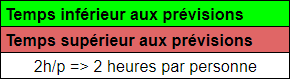
\includegraphics[width=0.4\textwidth]{./img/legende.PNG}}
    \caption{\label{} Légende tableaux Gantt}
\end{figure}


\begin{figure}[H]
\makebox[\textwidth][c]{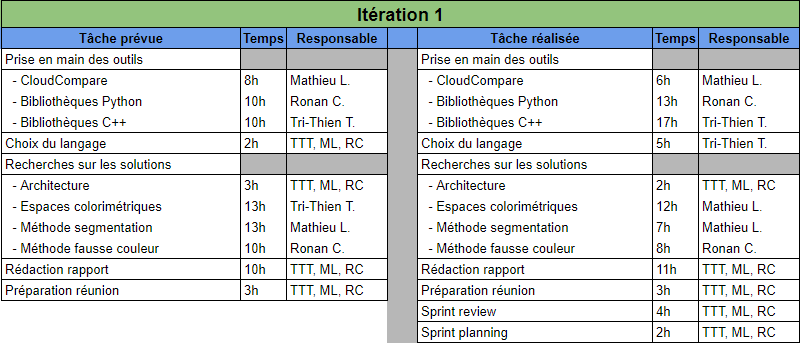
\includegraphics[width=1.2\textwidth]{./img/gantt_1.PNG}}
    \caption{\label{} Comparaison Gantt de l'itération 1}
\end{figure}

Ce premier tableau nous montre les tâches que nous avions prévues pour notre première itération, représentées du côté gauche, avec la tâche prévue, le temps estimé et le responsable de la tâche. De l'autre côté, nous pouvons observer les mêmes tâches, avec le temps réellement passé pour les réaliser. \newline

Nous pouvons voir que le temps réellement passé ne correspond pas du tout à ce que nous avions prévu. En effet, comme il s'agissait de notre première itération, il nous a été difficile d'estimer notre capacité de travail, et du temps à accorder à chacune de nos tâches. \newline

Nous pouvons aussi observer que sur la tâche des recherches sur les espaces colorimétriques, le responsable a été changé, de même que pour le choix du langage. Pendant notre avancée sur l'itération, nous nous sommes rendu compte que certaines tâches étaient plus rapide à réaliser que d'autres, par exemple sur la prise en main de CloudCompare, ou encore sur les méthodes de segmentation. Ce gain de temps nous a permis d'attribuer la responsabilité de travailler sur les espaces colorimétriques à Mathieu L, et libérer du temps à Tri-Thien T. Ce dernier a eu beaucoup de temps supplémentaire à attribuer sur ses tâches, notamment car il s'agit d'un travail de recherches, donc cela nécessite beaucoup de documentations, et par conséquent beaucoup de temps. Il fallait également produire un rapport facile à comprendre pour les autres membres du groupe, et pour le client. \newline

De plus, nous avions des tâches qui n'étaient pas prévues dans nos prévisions, mais qui étaient présentes en implicitement. Nous pouvons citer la préparation du Sprint review, ou encore le sprint planning. C'est pour cela que ces tâches n'apparaissent pas dans les tâches prévues, mais uniquement dans les tâches réalisées.

\begin{figure}[H]
\makebox[\textwidth][c]{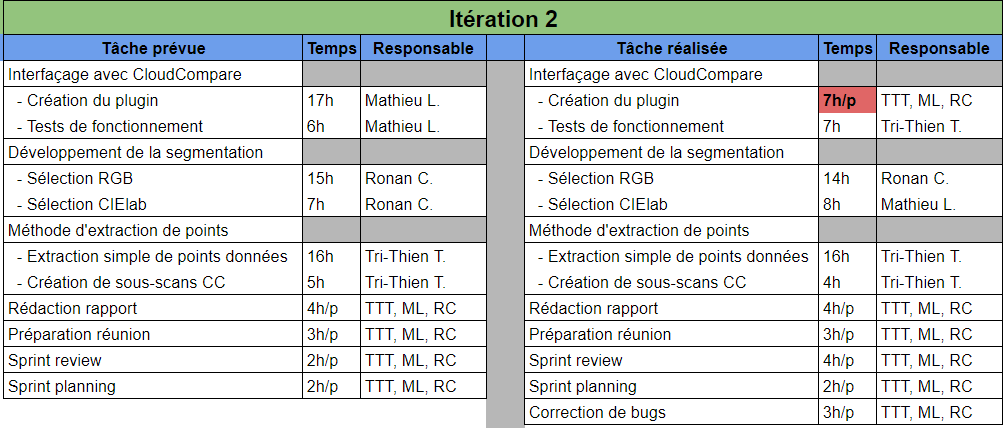
\includegraphics[width=1.2\textwidth]{./img/gantt_2.PNG}}
    \caption{\label{} Comparaison Gantt de l'itération 2}
\end{figure}

Pour la deuxième itération, les prévisions du nombre d'heures par tâches ont plutôt bien été respectées, sauf pour la partie sur l'interfaçage avec CloudCompare. En effet, cette partie était concentrée sur l'implémentation d'un nouveau plugin sur le logiciel CloudCompare. Nous avions un tutoriel à notre disposition pour l'installation, mais nous avions rencontré beaucoup de problèmes. Nous pouvons par exemple citer les différents logiciels à installer au préalable (QT, PCL...), qui sont très volumineux et prennent beaucoup de temps à installer. Ensuite, il faut savoir comment les utiliser, ce qui demande une phase de formation sur les outils. \newline

Une fois ceci fait, il fallait ensuite créer notre propre interface et nos propres algorithmes de traitement sur le nuage de points. Une fois encore, il fallait que l'on se forme sur comment un plugin CloudCompare fonctionne, sa structure et comment ajouter notre propre code.

\begin{figure}[H]
\makebox[\textwidth][c]{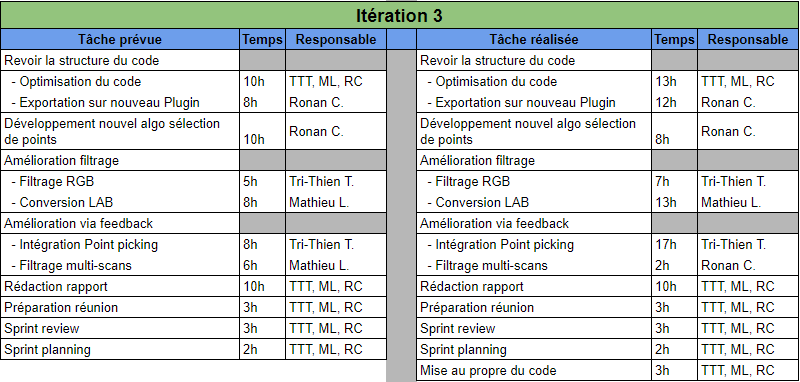
\includegraphics[width=1.2\textwidth]{./img/gantt_3.PNG}}
    \caption{\label{} Comparaison Gantt de l'itération 3}
\end{figure}

Cette troisième itération était dédiée à l'amélioration de notre solution, et surtout à revoir la structure de notre code pour avoir une meilleure organisation. De même que pour la première itération, nous avons eu ici du mal à bien estimer la durée de nos tâches. Les principales différences entre le prévisionnel et le réalisé est le fait que nous ne connaissons pas encore assez le code du projet CloudCompare, donc ne savons pas vraiment ce qui est possible de faire avec les outils du projet ou non. \newline

De plus, nous avons rencontré des difficultés pour obtenir des résultats satisfaisants, notamment pour la conversion LAB, et des difficultés à comprendre le fonctionnement d'un plugin sur le logiciel CloudCompare, notamment le principe des signaux et des slots en C++ (pour l'implémentation d'un point picking). \newline

Il faut aussi noter que pour le développement d'un nouvel algorithme de sélection de points dans le nuage, la durée indiquée ici ne veut pas dire que la tâche est terminée. En effet, la tâche est plus compliquée que prévu, et malgré le temps donné à cette tâche, il faut encore y attribuer du temps pour la finaliser.

\begin{figure}[H]
\makebox[\textwidth][c]{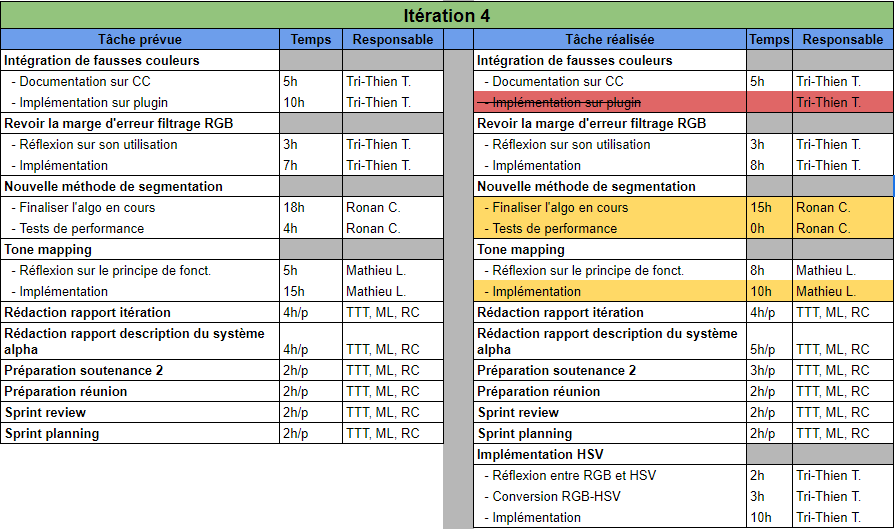
\includegraphics[width=1.2\textwidth]{./img/gantt_4.PNG}}
    \caption{\label{} Comparaison Gantt de l'itération 4}
\end{figure}

La quatrième itération était concentrée principalement sur l'avancement du développement des tâches. Nous pouvons noter que certaines tâches sont encore en cours, notamment la nouvelle méthode de segmentation, et le tone mapping. En effet, ces tâches sont longues et assez complexes à développer. La majeur partie du code est implémenté, mais il reste surtout une phase de déboggage à effectuer, pour que l'exécution soit fonctionnelle. \newline

Nous avions aussi remarqué pendant l'itération, que l'intégration de fausses couleurs n'était plus vraiment d'actualité. En effet, celle-ci était déjà présente sur le logiciel CloudCompare. Nous n'avions donc pas de plus-value à apporter sur cette fonctionnalité. \newline

Par la suite, nous avions trouvé un autre type de filtrage, que nous n'avions jusqu'à ce moment pas développé, qui est le fait d'utiliser un autre espace colorimétrique. Après avoir vu les limites du RGB, nous avons essayé de passer par le HSV afin d'avoir des meilleures bornes de couleurs. Nous avons donc ajouté cette tâche pour cette itération.

\begin{figure}[H]
\makebox[\textwidth][c]{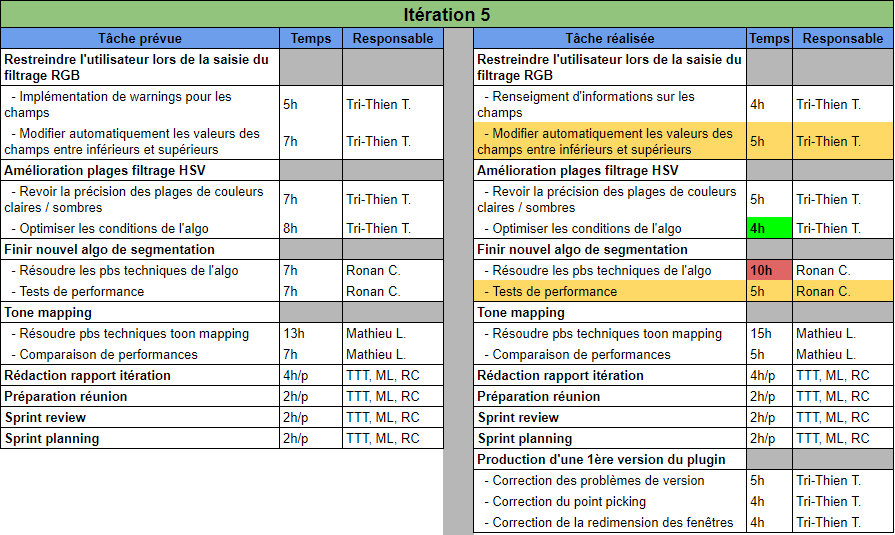
\includegraphics[width=1.2\textwidth]{./img/gantt_5.PNG}}
    \caption{\label{} Comparaison Gantt de l'itération 5}
\end{figure}

Pour la cinquième itération, nous avons pu faire une démonstration du filtrage HSV pour le client. Il fallait donc prendre en compte les retours et y apporter des améliorations. De plus, nous avions toujours des améliorations à apporter pour le filtrage RGB. La tâche concernant la production de la première version du plugin, n'était pas prévue au départ. Celle-ci a été plutôt compliquée avec les différents problèmes liés aux versions des logiciels, et des délais de communication. Il fallait aussi apporter des correctifs pour certains bugs apparus entre les différentes machines. \newline

Nous avions eu un peu plus de difficulté à respecter les temps prévus, car nous avions dû replanifier nos tâches avec l'annulation du projet icreate.

\begin{figure}[H]
\makebox[\textwidth][c]{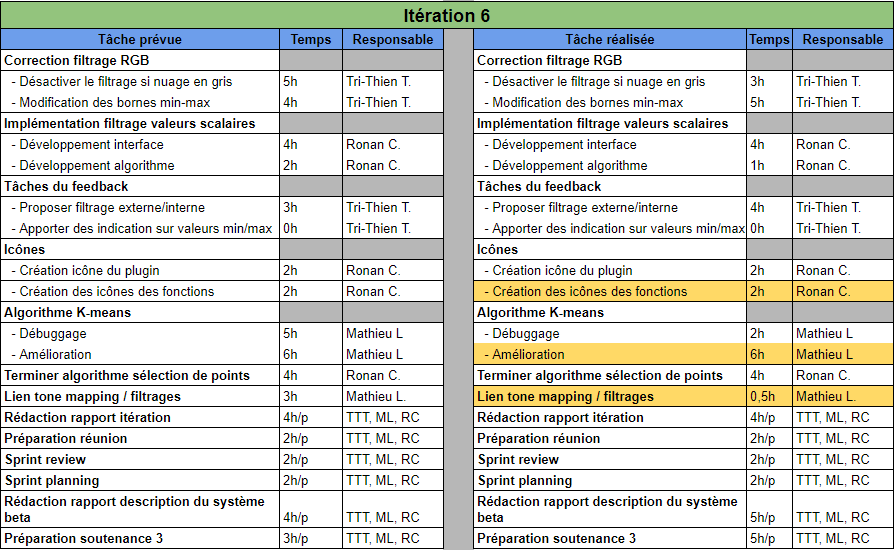
\includegraphics[width=1.2\textwidth]{./img/gantt_6.PNG}}
    \caption{\label{} Comparaison Gantt de l'itération 6}
\end{figure}

Lors de cette dernière itération, nous avons pu faire un point avec le client et notre tuteur académique. Cela nous a permis de valider nos nouvelles tâches implémentées, et de réfléchir à ce que l'on devait développer, par rapport au temps restant. En plus de ces tâches, il nous fallait aussi préparer notre dernière soutenance sur le système réalisé, version beta. \newline

La décision qui a été prise est que nous devions surtout nous concentrer sur la finalisation des tâches en cours (algorithme de sélection de points / tone mapping). De plus, il nous fallait passer du temps à la correction de bugs, ainsi qu'à l'amélioration des fonctionnalité vis à vis du feedback des utilisateurs. \newline

Durant cette itération, les temps prévus sont plutôt bien respectés par rapport à la réalisation. Cela pourrait venir du fait que nous avions pris l'habitude d'estimer notre capacité de travail, et qu'il nous était plus facile de travailler sur ce projet en cette période de confinement. En effet, nous avions moins de cours et plus de temps à accorder au projet transversal.

\subsection{Rapport de recette}

Ce rapport de recette va permettre d'avoir des retours sur l'installation du projet et des différentes fonctionnalités qui ont été développées / non développées.

\subsubsection {Installation}

Ce projet contient un code source avec le logiciel CloudCompare, et notre plugin. Ce dernier se situe dans le dossier "plugins". \newline

C'est un projet CMake, que nous générons avec la version 3.16.1 de CMake GUI. Une fois celui-ci généré, nous utilisons Visual Studio 15 (2017) pour la compilation, avec le SDK windows 10.0.17763.0. Le fichier généré sera "ColorimetricSegmenter.dll".\newline

Au niveau de l'installation côté client, il aura donc le fichier ".dll", qu'il faudra ajouter dans CloudCompare. Pour cela, il devra tout d'abord installer CloudCompare. La version 2.11.beta est une version qui permet de faire fonctionner notre plugin, mais les versions antérieures ne le permettent pas. Il faudra ensuite aller dans le répertoire d'installation (celui de base est "C:\textbackslash Program Files\textbackslash CloudCompare"), et insérer le fichier ".dll" dans le sous-dossier "plugins". \newline

Une fois que CloudCompare est lancé, il est maintenant possible de voir notre plugin ColorimetricSegmenter dans l'onglet Plugins, et aussi les icônes dans la barre de raccourcis. \newline

Nous avions rencontré des problèmes de compatibilité lorsque nous compilions avec une version plus récente de Visual Studio (2019), et donc une version du SDK windows plus récente. Certaines machines avec d'anciennes mise à jour de windows ne pouvaient pas faire fonctionner le plugin. En utilisant la version 2017 de Visual Studio, ce problème a été résolu.

\subsubsection {Résultats des User Stories}

Lors de la réalisation du cahier des charges, nous avions prévu des User Stories, afin de décrire en détail le fonctionnement de nos fonctionnalités. Suite au rapport de sprint review de l'itération 2, nous avions décidé, avec la recommandation et l'accord du client et du tuteur académique, de passer sur un plugin pour CloudCompare. Cette décision permettait d'utiliser un outil complet et spécialisé dans le domaine du traitement de nuage de points, donc de nous éviter de développer des fonctionnalités déjà existantes sur d'autres outils. Certaines User Stories ont donc été modifiées, notamment la lecture d'un nuage de points et l'exportation, pour être remplacé par l'implémentation d'un nouveau plugin sur CloudCompare. Les nouvelles User Stories du sprint review sont les suivantes :

\begin{itemize}
  \item US1 : Intégrer un plugin CloudCompare
  \item US2 : Isoler un élément dans le nuage de points, selon sa plage de couleur
  \item US3 : Créer des sous-scans suite au filtrage\\
\end{itemize}

Au niveau des tests d'acceptation, il faut noter que comme nous les avions rédigé au début de projet, nous ne savions pas vraiment comment nos fonctionnalités allaient se dérouler. Certains scénarios peuvent donc être différents par rapport à ce que nous avons maintenant. Ces tests d'acceptation, par User Story, sont les suivants : \\

\textbf{\og US1 : Intégrer un plugin CloudCompare\fg{}}

En tant qu'utilisateur du logiciel CloudCompare, je souhaite voir dans la liste des plugins, un nouveau filtre personnalisé afin d'y ajouter un nouvel algorithme de segmentation.

\textbf{Tests d'acceptation :}

\begin{enumerate}
    \item \textbf{Scénario 1}

Étant donné que je suis sur le logiciel CloudCompare\\
Quand j'affiche la liste des plugins\\
Alors un nouveau bouton du filtre personnalisé apparaît\\
Alors les fonctionnalités dans le plugin sont désactivées\\

    \item \textbf{Scénario 2}

Étant donné que je suis sur le logiciel CloudCompare\\
Quand j'importe un nuage de points \\
Quand je sélectionne le scan correspondant \\
Quand j'affiche la liste des plugins\\
Alors les fonctionnalités dans le plugin sont activées\\
\end{enumerate}

\begin{figure}[H]
\makebox[\textwidth][c]{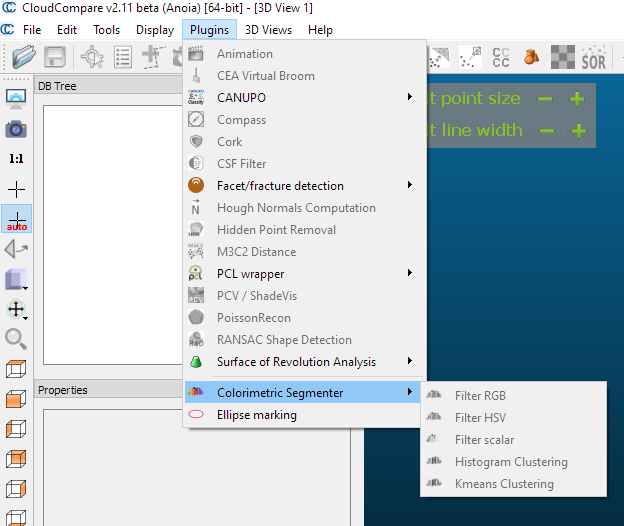
\includegraphics[width=0.7\textwidth]{./img/us1_1.PNG}}
    \caption{\label{} Résultat US1 - S1}
\end{figure}

Dans cette image, nous pouvons voir l'implémentation de notre plugin dans le logiciel CloudCompare. Lorsqu'aucun scan n'est sélectionné, nos fonctionnalités sont bien désactivées.

\begin{figure}[H]
\makebox[\textwidth][c]{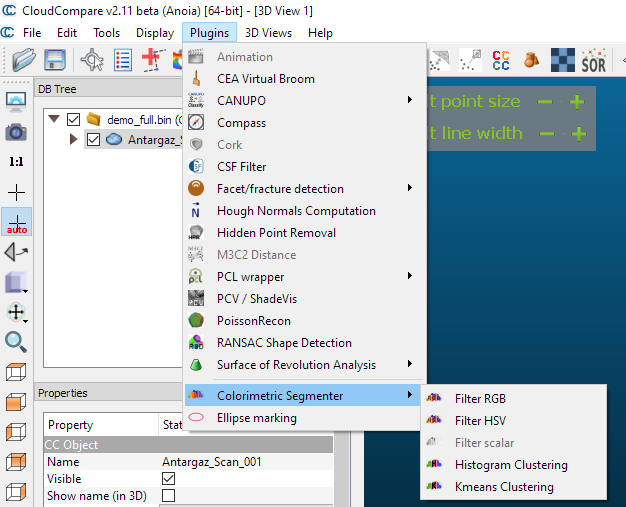
\includegraphics[width=0.7\textwidth]{./img/us1_2.PNG}}
    \caption{\label{} Résultat US1 - S2}
\end{figure}

Lorsqu'un nuage de points a été importé et sélectionné en tant que scan, certains de nos algorithmes s'activent. Ici, la fonctionnalité "Filter scalar" ne peut pas s'activer, car le nuage de points contient des points avec des valeurs RGB. Dans l'User Story 1, les cas sont donc passants. \newline

\textbf{\og US2 : Isoler un élément dans le nuage de points, selon sa plage de couleur\fg{}}

En tant qu'utilisateur du logiciel, je souhaite isoler un élément dans le nuage de points afin d'afficher à l'écran uniquement l'élément voulu selon sa couleur.

\textbf{Tests d'acceptation :}
\begin{enumerate}

    \item \textbf{Scénario 1}

Étant donné que j'ai affiché un nuage de points via un fichier\\
Quand je clique sur l'option pour isoler un élément\\
Alors une interface avec un color picker apparaît\\
Quand je sélectionne une plage de couleur\\
Et que je clique sur le bouton de validation\\
Alors l'interface disparaît\\
Et le nuage de points n'affiche uniquement que les points respectant la plage d'intensité de couleur.

    \item \textbf{Scénario 2}

Étant donné que j'ai affiché un nuage de points via un fichier\\
Quand je clique sur l'option pour isoler un élément\\
Alors une interface avec un color picker apparaît\\
Quand je sélectionne une plage de couleur\\
Et que je clique sur le bouton d'annulation\\
Alors l'interface disparaît\\
\end{enumerate}

Sur ces scénarios, nous avions prévu d'utiliser un color picker pour permettre à l'utilisateur de choisir la couleur qu'il veut filtrer. Suite aux feedbacks, le client préférait une solution où il était possible de cliquer sur un point dans le nuage, et d'automatiquement récupérer sa couleur. Cette fonctionnalité s'appelle le "point picking". \newline

Sur cet exemple d'interface dans l'image \ref{ui_hsv}, nous pouvons voir qu'il est possible d'utiliser le point picking, via le bouton à gauche de la fenêtre. Les boutons de validation ou d'annulation sont les boutons "OK" et "Cancel". Si l'utilisateur clique sur le bouton Cancel, rien ne se passe, et s'il clique sur le bouton OK, un nouveau nuage de points apparaît, avec le résultat du filtrage \ref{application_hsv}. Ces scénarios sont donc passants, même s'il y a eu quelques modifications. \newline

\textbf{\og US3 : Créer des sous-scans suite au filtrage\fg{}}

En tant qu'utilisateur du logiciel, je souhaite créer des sous-scans après filtrage, afin de séparer les points externes et les points internes à la sélection.

\textbf{Tests d'acceptation :}
\begin{enumerate}

    \item \textbf{Scénario 1}

Étant donné que j'ai affiché un nuage de points via un fichier\\
Quand je clique sur le bouton pour filtrer mon nuage de points\\
Alors une interface de paramètres apparaît\\
Quand je valide les paramètres\\
Alors l'interface disparaît\\
Alors des sous-scans s'affichent dans la liste des scans
\end{enumerate}

\begin{figure}[H]
\makebox[\textwidth][c]{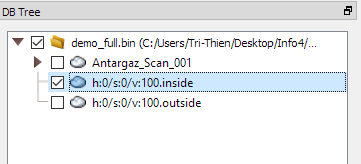
\includegraphics[width=0.5\textwidth]{./img/us3_1.png}}
    \caption{\label{} Résultat US3 - S1}
\end{figure}

Lorsque l'utilisateur valide une fenêtre d'un filtrage (ici le HSV par exemple), la fenêtre disparaît pour revenir sur un nouveau scan, celui qui est automatiquement sélectionné, et donc affiché sur le logiciel. Le scan original est encore présent (Antargaz\_Scan\_001), et un ou plusieurs sous-scans apparaissent, avec des noms qui affichent les paramètres utilisés selon le type de filtrage. Ce test d'acceptation valide donc notre troisième User Story.

\subsubsection {Recette fonctionnelle du commanditaire}

Toutes nos fonctionnalités ont été testées et validées par le client. il a pu tester nos algorithmes sur des cas réelles de nuage de points, et nous faire remonter certains problèmes, que nous avons pour la plupart corrigés.
% TODO parler du tone mapping

\subsubsection {Fonctionnalités du cahier des charges non développées / non validées}

% TODO Algo sélection de points

% TODO Tone mapping K-means ?

\newpage
\begin{thebibliography}{3}
	\bibitem{cc} Présentation de Cloud Compare: \url{https://www.danielgm.net/cc/}
	\bibitem{3DList} Liste regroupant les principales bibliothèques 3D: \url{https://github.com/openMVG/awesome_3DReconstruction_list#mesh-storage-processing}
	\bibitem{PCL} Présentation de PCL: \url{http://www.pointclouds.org/}
	\bibitem{Open3D} Présentation de Open3D: \url{http://www.open3d.org/}
	\bibitem{PDAL} Présentation de PDAL: \url{https://pdal.io/index.html}
	\bibitem{seg} Punya Prasad Sapkota, \textit{Segmentation of Coloured Point Cloud Data}, 2008 \url{https://pdfs.semanticscholar.org/efdb/3ff43d5beffa3845e6434b580f775e2abf85.pdf}
	\bibitem{seg1} Erzhuo Che, Jaehoon Jung, et Michael J. Olsen, \textit{Object Recognition, Segmentation, and Classification of Mobile Laser Scanning Point Clouds: A State of the Art Review}, 2019
	\bibitem{B01} Qingming Zhan, Yubin Liang, Yinghui Xiao, \textit{Color-based segmentation of point clouds}, 2009 \url{https://www.researchgate.net/profile/Q_Zhan/publication/228917371_Color-based_segmentation_of_point_clouds/links/09e4150cd7253dcafa000000/Color-based-segmentation-of-point-clouds.pdf}
  	\bibitem{B02} Conversion RGB - HSV : \url{https://mattlockyer.github.io/iat455/documents/rgb-hsv.pdf}
\end{thebibliography}
\end{document}
